\documentclass[border=10pt,varwidth]{standalone}
\usepackage{tikz}
\usetikzlibrary{shapes,arrows,shapes.multipart, positioning}

\begin{document}

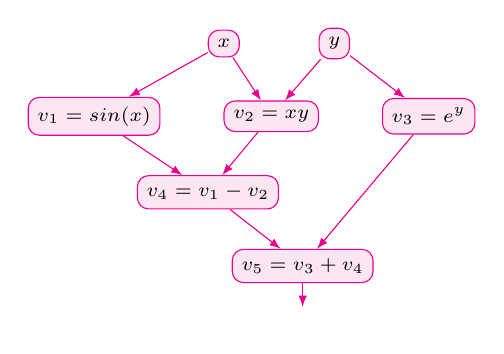
\begin{tikzpicture}
    \tikzset{
        node/.style = {rectangle, draw=magenta,  fill=magenta!10, thin, rounded corners},
        line/.style = {draw=magenta, thin, -latex}
    }

    \node[node](x){\scriptsize{$x$}};
    \node[node](y)[right = 1.0cm of x]{\scriptsize{$y$}};

    \node[node](sinx)[below left = 0.5 and 0.6cm of x]{\scriptsize{$v_1=sin(x)$}};
    \node[node](xy)[right = 0.8cm of sinx]{\scriptsize{$v_2=xy$}};
    \node[node](expy)[right = 0.8cm of xy]{\scriptsize{$v_3=e^y$}};


    \node[node](minus)[below right = 0.5cm and -0.3cm of sinx]{\scriptsize{$v_4=v_1 - v_2$}};

    \node[node](plus)[below right = 0.5cm and -0.6cm of minus]{\scriptsize{$v_5=v_3 + v_4$}};

    \node(end)[below =0.3cm of plus]{};

    \path [line] (x) -- (sinx);
    \path [line] (x) -- (xy);

    \path [line] (y) -- (xy);
    \path [line] (y) -- (expy);

    \path [line] (sinx) -- (minus);
    \path [line] (xy) -- (minus);

    \path [line] (expy) -- (plus);
    \path [line] (minus) --  (plus);
    \path [line] (plus) --(end);

\end{tikzpicture}

\end{document}
